% !TEX TS-program = pdflatex
% !TEX encoding = UTF-8 Unicode

\documentclass[a4paper, titlepage=false, parskip=full-, 10pt]{scrartcl}

\usepackage[utf8]{inputenc}
\usepackage[T1]{fontenc}
\usepackage[english, ngerman]{babel}
\usepackage{babelbib}
\usepackage{hyperref}
\usepackage{listings}
\usepackage{framed}
\usepackage{color}
\usepackage{graphicx}
\usepackage[normalem]{ulem}
\usepackage{cancel}
\usepackage{array}
\usepackage{amsmath}
\usepackage{amssymb}
\usepackage{amsthm}
\usepackage{algorithm}
\usepackage{algorithmic}
\usepackage{geometry}
\usepackage{subfigure}
\geometry{a4paper, top=20mm, left=35mm, right=25mm, bottom=40mm}

\newcounter{tasknbr}
\setcounter{tasknbr}{1}
\newenvironment{task}[1]{{\bf Aufgabe \arabic {tasknbr}\stepcounter{tasknbr}} (#1):\begin{enumerate}}{\end{enumerate}}
\newcommand{\subtask}[1]{\item[#1)]}

% Listings -----------------------------------------------------------------------------
\definecolor{red}{rgb}{.8,.1,.2}
\definecolor{blue}{rgb}{.2,.3,.7}
\definecolor{lightyellow}{rgb}{1.,1.,.97}
\definecolor{gray}{rgb}{.7,.7,.7}
\definecolor{darkgreen}{rgb}{0,.5,.1}
\definecolor{darkyellow}{rgb}{1.,.7,.3}
\lstloadlanguages{C++,[Objective]C,Java}
\lstset{
escapeinside={§§}{§§},
basicstyle=\ttfamily\footnotesize\mdseries,
columns=fullflexible,
keywordstyle=\bfseries\color{blue},
commentstyle=\color{darkgreen},      
stringstyle=\color{red},
numbers=left,
numberstyle=\ttfamily\scriptsize\color{gray},
breaklines=true,
showstringspaces=false,
tabsize=4,
captionpos=b,
float=htb,
frame=tb,
frameshape={RYR}{y}{y}{RYR},
rulecolor=\color{black},
xleftmargin=15pt,
xrightmargin=4pt,
aboveskip=\bigskipamount,
belowskip=\bigskipamount,
backgroundcolor=\color{lightyellow},
extendedchars=true,
belowcaptionskip=15pt}

%% Enter current values here: %%
\newcommand{\lecture}{Robotik WS15/16}
\newcommand{\tutor}{}
\newcommand{\assignmentnbr}{5}
\newcommand{\students}{Julius Auer, Thomas Tegethoff}
%%-------------------------------------%%

\begin{document}  
{\small \textsl{\lecture \hfill \tutor}}
\hrule
\begin{center}
\textbf{Übungsblatt \assignmentnbr}\\
[\bigskipamount]
{\small \students}
\end{center}
\hrule

\begin{task}{Umzug nach ROS-Indigo}
\item[]
... ist schon letzte Woche erfolgt.
\end{task}

\begin{task}{Roboter-Simulator Gazebo}
\item[]
Wir sollen Screenshots erzeugen und zwar:

- \emph{einen der simulierten Punktwolke (in rviz)}

Folgt man dem Tutorial:

\url{http://wiki.ros.org/laser_pipeline/Tutorials/IntroductionToWorkingWithLaserScannerData}

sollte eine LaserScan-Message von rviz interpretiert werden können. Dies ist (hier bei uns) jedoch nicht der Fall: das Laser-Plugin liefert den in Abbildung \ref{fig:2-1} gezeigten Fehler. Das eine korrekte SensorMsg von gazebo gepublished wird, ist hierbei durch \emph{rostopic info} geprüft worden. Dokumentiert sind die meisten ros-Sachen ja bekanntlich katastrophal - so findet man auch hier reichlich tote links (z.B.

\url{http://pr.willowgarage.com/pr-docs/ros-packages/laser_scan/html/classlaser__geometry_1_1LaserProjection.html}

) wenn man nach Paket-Dokus sucht. Das macht Probleme sehr schwer zu debuggen und erneut haben wir somit eine Situation, die wir ohne signifikanten Zeitaufwand nicht lösen können. Sehr ärgerlich (und zeitaufwändig!). Den Beweis, dass wir den Sensor sinnvoll montiert haben, liefert Abbildung \ref{fig:2-2}.

\begin{figure}[!htpb]
\centering
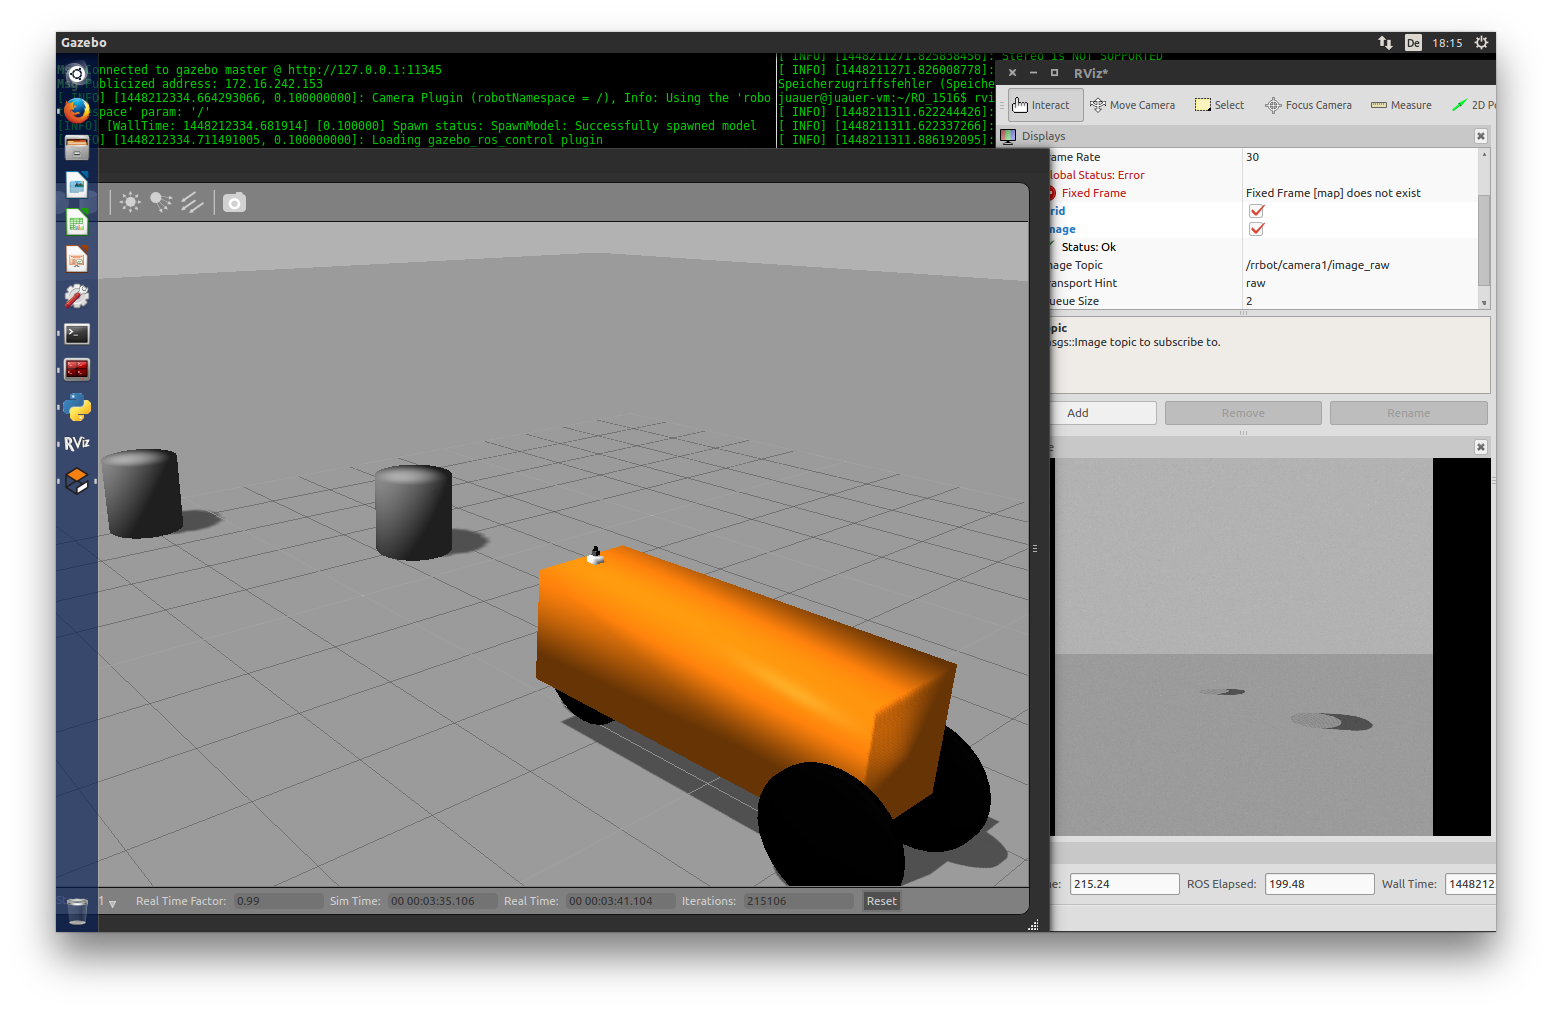
\includegraphics[width=0.6\linewidth]{capture_2-1}
\label{fig:2-1}
\caption{Fehler}
\end{figure}

\begin{figure}[!htpb]
\centering
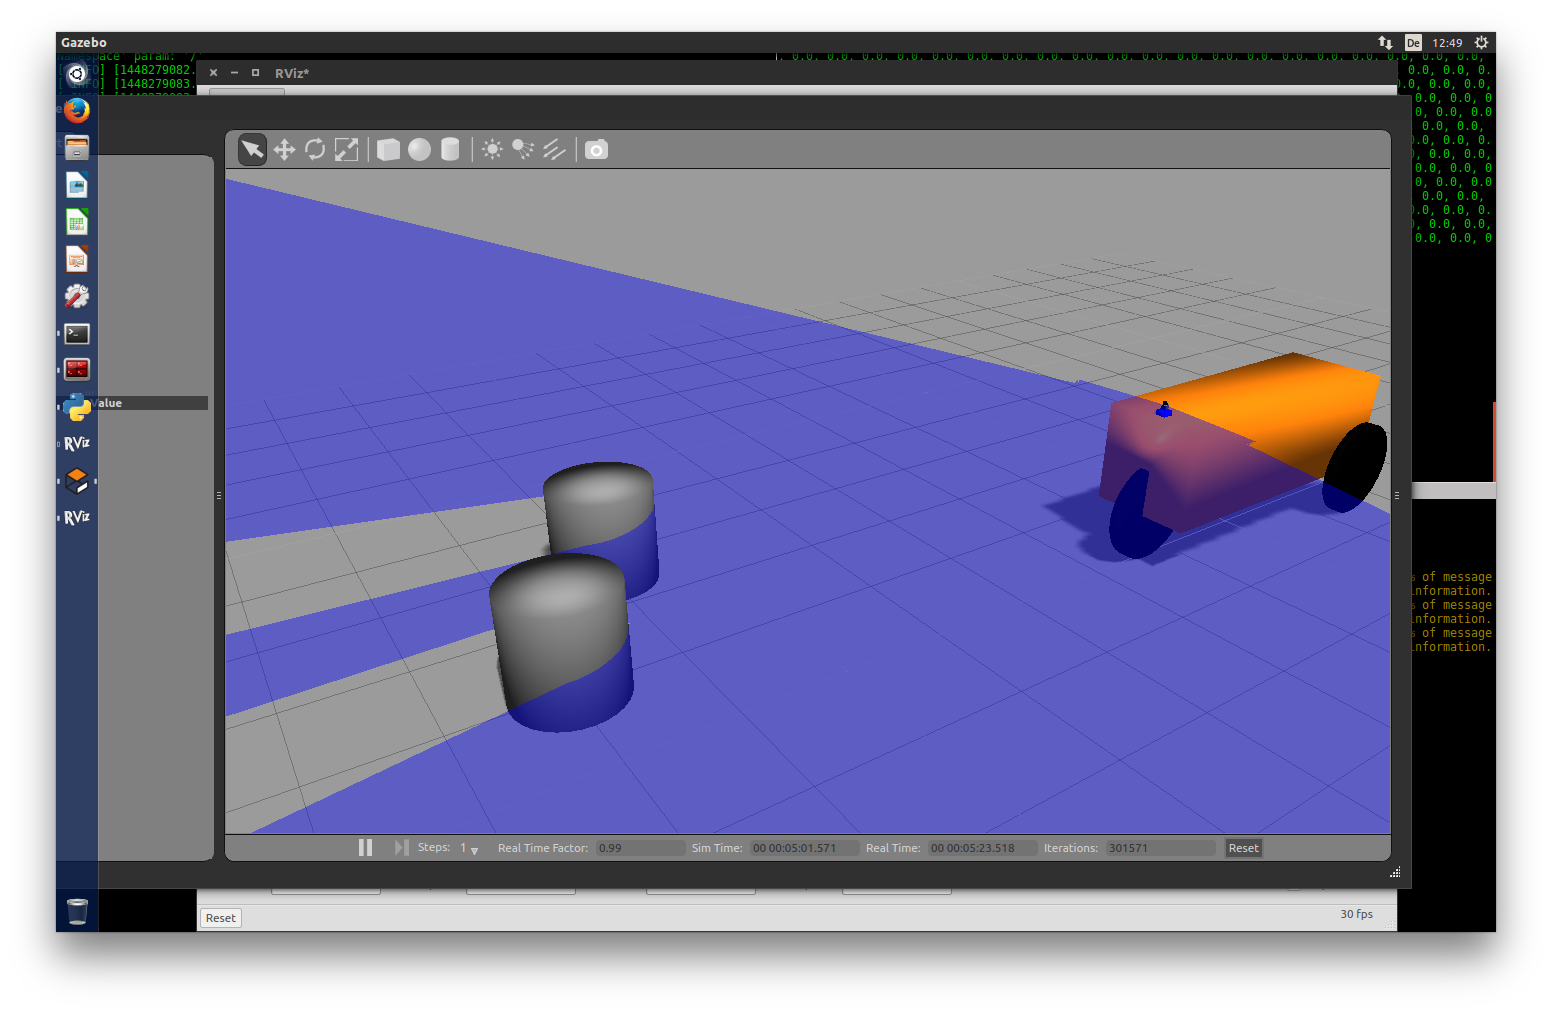
\includegraphics[width=0.8\linewidth]{capture_2-2}
\label{fig:2-2}
\caption{Roboter mit Laser}
\end{figure}

\newpage
- \emph{einen mit dem simulierten Kamerabild (in gazebo)}

Wie man in gazebo ein Kamerabild anzeigen kann wird {\bf nirgends} erwähnt. Im Tutorial und den anderen ''offiziellen'' Kanälen werden ein \emph{image\_show} Paket und rviz empfohlen. Nach ausgiebiger (und wieder zeitaufwändiger!) Suche kommen wir zu dem Schluss, dass gazebo kein Kamerabild anzeigen kann und die Aufgabe nicht zu lösen ist.

Nun, das beste (und m.E. auch das sinnvollste!) was wir hier anbieten können, ist ein Kamerabild in rviz (siehe auch Abbildung \ref{fig:2-3}) über das Image-Display. Aus irgendeinem Grund haben die Objekte manchmal eine z-Ausdehnung, manchmal aber auch nicht.

\begin{figure}[!htpb]
\centering
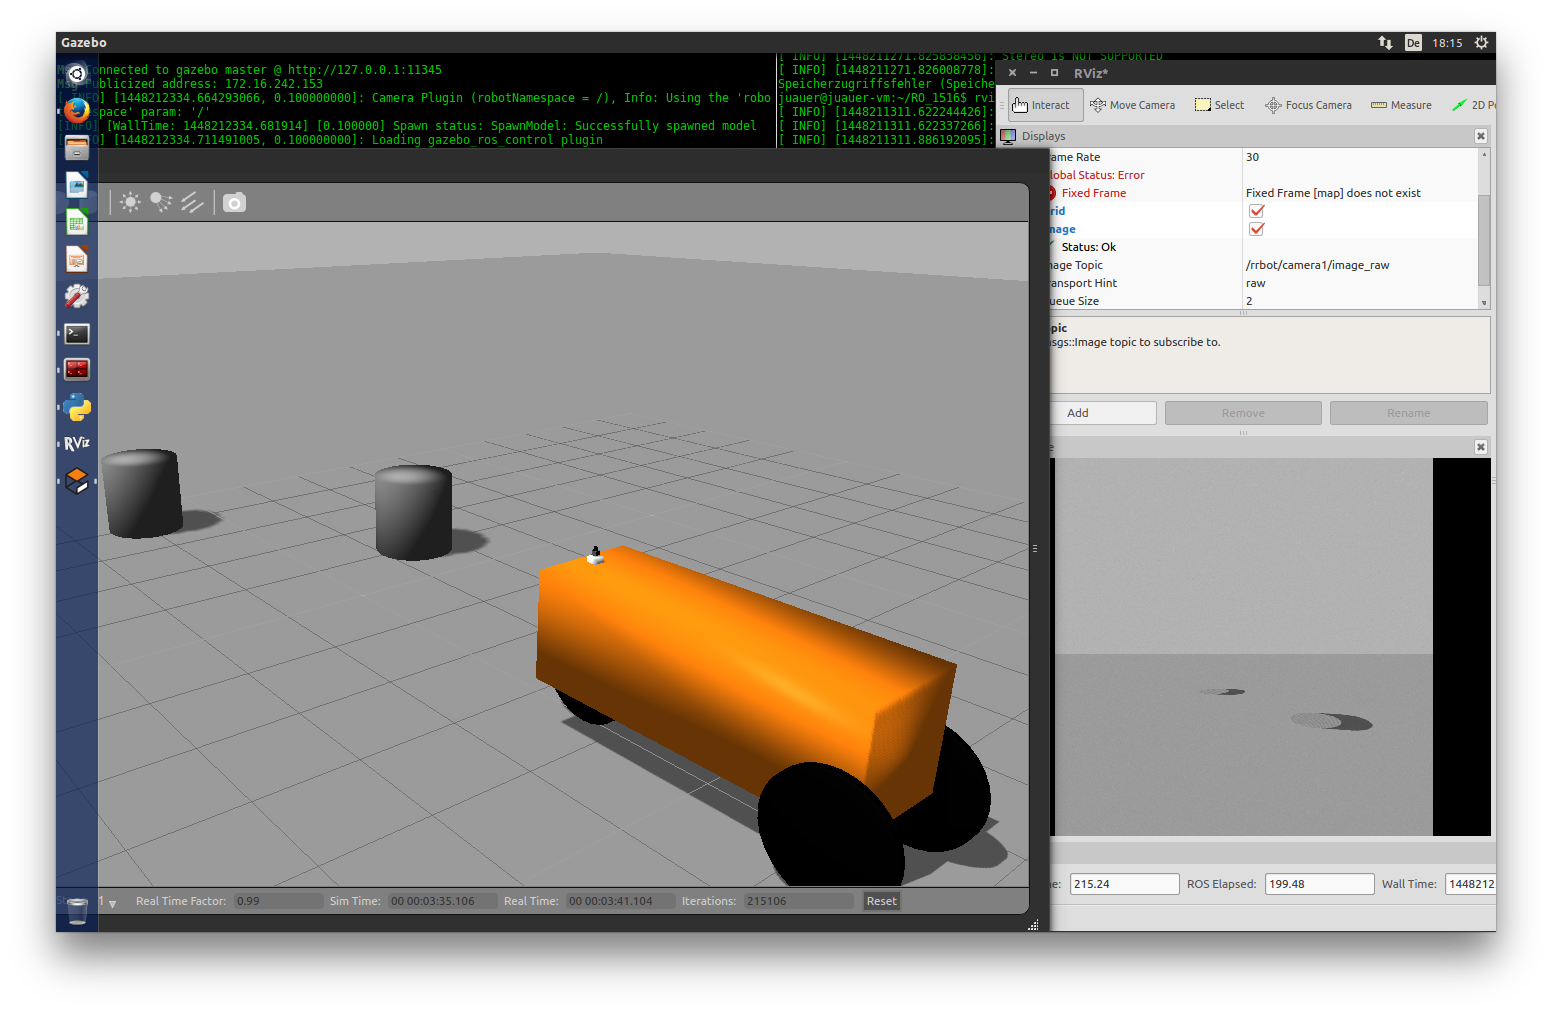
\includegraphics[width=0.8\linewidth]{capture_2-3}
\label{fig:2-3}
\caption{Roboter mit Kamera und (obendrauf) Laser in gazebo (links) und Kamerabild in rviz (rechts)}
\end{figure}
\end{task}

\begin{task}{DH-Parameter}
\item[]
\begin{table}[!htpb]
\centering
\begin{tabular}{>{$}c<{$}|>{$}c<{$}>{$}c<{$}>{$}c<{$}>{$}c<{$}}
i	&	d	&	\theta	&	a	&	\alpha\\\hline
1	&	L_1	&	\theta_1	&	0	&	0\\
2	&	0	&	\theta_2	&	0	&	\frac{\pi}{2}\\
3	&	0	&	\theta_3	&	L_2	&	0
\end{tabular}
\end{table}

Config. shown: $\theta_1=160,\theta_2=45,\theta_3=20$

Transformation von \{3\} nach \{2\}:

\begin{align*}
T_{\{3\}\rightarrow\{2\}}=\begin{pmatrix}c\theta_3&-s\theta_3&0&L_2\cdot c\theta_3\\
s\theta_3&c\theta_3&0&L_2\cdot s\theta_3\\
0&0&1&0\\
0&0&0&1\end{pmatrix}
\end{align*}

Plausibilitäts-Test:\\
Seien: $\theta =\frac{\pi}{2},L_2=1,x_{\{3\}}=\begin{pmatrix}1\\1\\0\end{pmatrix}$\\
Erwartung: $T_{\{3\}\rightarrow\{2\}}\cdot x_{\{3\}}=\begin{pmatrix}-1\\2\\0\end{pmatrix}$

\begin{align*}
\begin{pmatrix}c\left(\frac{\pi}{2}\right)&-s\left(\frac{\pi}{2}\right)&0&c\left(\frac{\pi}{2}\right)\\
s\left(\frac{\pi}{2}\right)&c\left(\frac{\pi}{2}\right)&0&s\left(\frac{\pi}{2}\right)\\
0&0&1&0\\
0&0&0&1\end{pmatrix}\cdot\begin{pmatrix}1\\1\\0\\1\end{pmatrix}&=\begin{pmatrix}0-1+0+0\\1+0+0+1\\0+0+0+0\\0+0+0+1\end{pmatrix}=\begin{pmatrix}-1\\2\\0\\1\end{pmatrix}
\end{align*}

$\rightarrow$ Super.
\end{task}

\begin{task}{Jacobi-Matrix}
\subtask{a}
\begin{align*}
	x &= q_{3}*\cos(q_{1})\\
	y &= q_{3}*\sin(q_{1})\\
	z &= q_{2}
\end{align*}
\subtask{b}
\begin{align*}
	f(q_{1}) &= f(q_{2}) = f(q_{3}) = q_{3}*\cos(q_{1})\\
	g(q_{1}) &= g(q_{2}) = g(q_{3}) = q_{3}*\sin(q_{1})\\
	h(q_{1}) &= h(q_{2}) = h(q_{3}) = q_{2}\\
	\\
	f(q_{1})' &= q_{3}*-\sin(q_{1})\\
	f(q_{2})' &= 0\\
	f(q_{3})' &= \cos(q_{1})\\
	g(q_{1})' &= q_{3}*\cos(q_{1})\\
	g(q_{2})' &= 0\\
	g(q_{3})' &= \sin(q_{1})\\
	h(q_{1})' &= 0\\
	h(q_{2})' &= 1\\
	h(q_{3})' &= 0
\end{align*}
\subtask{c}
\begin{align*}
	\begin{pmatrix}
		q_{3}*-\sin(q_{1})	& q_{3}*\cos(q_{1})	& 0\\
		0					& 0					& 1\\
		\cos(q_{1})			& \sin(q_{1})		& 0
	\end{pmatrix}
\end{align*}
\end{task}
\end{document}
